\chapter{黑洞、白洞与整体因果图}

\lectureoverview{视界在局部是普通的，在整体上却是决定性的。我们从近视界施瓦西度规出发，借助欧几里得雪茄的类比向外推进，然后追问爱丽丝和鲍勃实际上能看到什么。奇点以及时间反演的白洞区域把这一局部图像扩展为永恒的施瓦西时空。彭罗斯紧致化使因果结构变得有限而可读。最后一步则从永恒解转向由坍缩形成的黑洞，其中牛顿球壳定理和伯克霍夫定理提供了需要拼接起来的各个部分。}

\section{从视界到无穷远}

在足够大的施瓦西视界附近，曲率在一个小实验室范围内是弱的，径向-时间几何近似为平坦的。方便的径向变量不是施瓦西坐标\(r\)，而是沿等时空间切片从视界向外测量的固有距离\(\rho\)：
\begin{equation}
\rho=0 \quad\Longleftrightarrow\quad r=2GM .
\label{eq:l04-rho-horizon}
\end{equation}
方便的时间坐标是无量纲量
\begin{equation}
\omega=\frac{t}{4GM},
\label{eq:l04-omega}
\end{equation}
其中\(c=1\)。因此，\(\omega\)是以两倍施瓦西半径为单位的施瓦西时间。

在mostly-plus约定下，近视界径向-时间度规为
\begin{equation}
ds^2\approx-\rho^2d\omega^2+d\rho^2.
\label{eq:l04-rindler}
\end{equation}
角向二维球面已被略去，因为当前的论证只涉及时间和径向距离。

\begin{figure}[htbp]
\centering
\includegraphics[width=0.72\textwidth]{lecture_04_figure_02.png}
\caption{近视界度规与重新标度的施瓦西时间。}
\lectureframe{00:05:46.800}
\end{figure}

方程~\eqref{eq:l04-rindler}与闵可夫斯基时空的关系，正如极坐标与欧几里得平面的关系。对于
\begin{equation}
T=\rho\sinh\omega,
\qquad
X=\rho\cosh\omega,
\end{equation}
可得
\begin{equation}
-dT^2+dX^2=-\rho^2d\omega^2+d\rho^2.
\end{equation}
常数\(\rho\)的线是双曲线\(X^2-T^2=\rho^2\)，而\(\omega\)从遥远的过去延伸到遥远的未来。两条零线\(X=\pm T\)在约化图的分叉点相交。在四维中，该点代表一个二维球面，而未来和过去的零面构成分叉的基灵视界。\editorialnote{只把交点称为分叉视界，在径向图中是有用的简略说法。更确切地说，两支视界分支相交于一个分叉二维球面。}

\subsection{远处区域}

施瓦西度规的径向-时间部分为
\begin{equation}
ds^2
=-\left(1-\frac{2GM}{r}\right)dt^2
+\frac{dr^2}{1-\frac{2GM}{r}}.
\label{eq:l04-schwarzschild}
\end{equation}
远离黑洞处，\(r\gg2GM\)，度规趋近于
\begin{equation}
ds^2\approx-dt^2+dr^2.
\end{equation}
在那里，\(r\)与\(\rho\)只相差一个无关紧要的加性修正，因此取\(dt=4GM\,d\omega\)，
\begin{equation}
ds^2\approx-(4GM)^2d\omega^2+d\rho^2.
\label{eq:l04-far}
\end{equation}
径向系数在两个极限下都很简单。发生变化的是时间系数：
\begin{equation}
ds^2\approx
\begin{cases}
-\rho^2d\omega^2+d\rho^2, & \rho\ll GM,\\[3pt]
-(4GM)^2d\omega^2+d\rho^2, & \rho\gg GM.
\end{cases}
\label{eq:l04-two-limits}
\end{equation}
沿悬停轨迹，\(d\rho=0\)。靠近视界处，
\begin{equation}
d\tau=\rho\,d\omega,
\end{equation}
而在远处\(d\tau\approx4GM\,d\omega=dt\)。对于外部时间坐标的固定增量，越靠近视界被保持的时钟所经历的固有时间越少。

\subsection{雪茄}

时空难以想象，因此把类时方向替换为普通的角方向。写
\begin{equation}
\begin{aligned}
d\ell^2&=F(\rho)^2d\theta^2+d\rho^2,\\
F(\rho)&\sim
\begin{cases}
\rho, & \rho\to0,\\
4GM, & \rho\to\infty.
\end{cases}
\end{aligned}
\label{eq:l04-cigar}
\end{equation}
在\(\rho=0\)附近，这就是极坐标中的平面。在远处，周长不再随半径增长：
\begin{equation}
C_\infty=\int_0^{2\pi}4GM\,d\theta=8\pi GM.
\label{eq:l04-cigar-circumference}
\end{equation}
因此该曲面在一端圆滑收拢，在另一端趋近于圆柱面。它看起来像一支雪茄。

\begin{figure}[htbp]
\centering
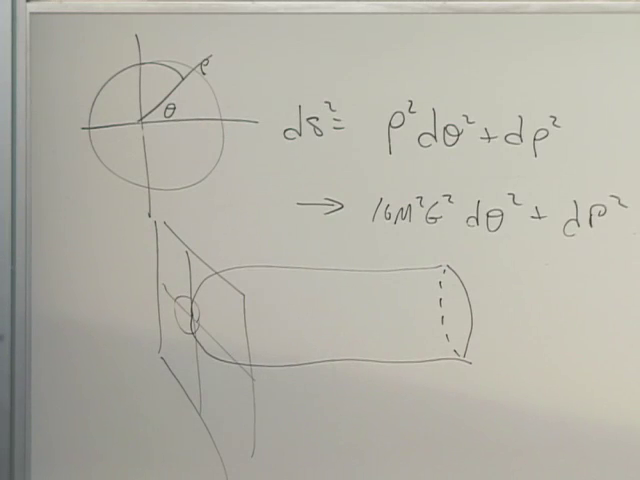
\includegraphics[width=0.74\textwidth]{lecture_04_figure_03.png}
\caption{欧几里得类比：一个极坐标尖端连接到一个周长为\(8\pi GM\)的渐近圆柱面。}
\lectureframe{00:14:05.000}
\end{figure}

质量越大，渐近处的围长越大，尖端附近的弯曲越平缓。小黑洞对应弯曲得很紧的雪茄；大黑洞则有一个宽阔、弯曲很弱的尖端。这是方程~\eqref{eq:l04-two-limits}中插值的图像，而不是洛伦兹黑洞本身的嵌入。\editorialnote{精确的几何对象是通过将施瓦西时间延拓到虚时间而得到的。于是尖端处的光滑性把欧几里得时间周期固定为\(8\pi GM\)，这同一个尺度后来决定了霍金温度。本讲在此只使用视觉类比。}

\section{从因果角度解读视界}

在黑洞外部，\(\rho>0\)，静止观测者沿一条常数\(\rho\)的双曲线运动。在远处，只需适度的加速度就能抵抗引力；靠近视界处，所需的固有加速度无界增长。一旦某条世界线穿过未来零边界，来自它的任何未来指向的因果信号都无法到达外部。

\begin{classroomqa}
\audiencequestion{在这个图上，光线是直线吗？\lecturetimestamp{00:20:21}}
\lecturerresponse{径向光线画在\(45^\circ\)处，除非另有约定。入射光线穿过视界；而已经在内部的出射光线无法再穿回外部。}
\end{classroomqa}

\begin{classroomqa}
\audiencequestion{入射光线会停留在视界上吗？\lecturetimestamp{00:21:12}}
\lecturerresponse{不会。向内瞄准的光线会穿过未来视界并继续进入黑洞内部。只有视界生成元本身才停留在零边界上。}
\end{classroomqa}

\subsection{Bob观察Alice}

让Bob在外部固定半径处悬停，而Alice向内下落。Bob只有通过接收来自Alice的向外传播的光才能看到她。假设她按照自己的时钟周期性地挥手。在她下落过程中较晚发出的信号需要越来越长的Schwarzschild时间才能到达Bob，而他每单位时间接收到的波越来越少。在穿过视界之后发出的任何信号都无法返回他那里。

Rindler坐标揭示了极限行为。定义出射零坐标
\begin{equation}
U=T-X=-\rho e^{-\omega}.
\end{equation}
趋近未来视界意味着\(U\to0^{-}\)，这要求在固定的外部\(\rho\)下\(\omega\to+\infty\)。因此，对Alice而言有限的穿越事件被推到了无限的外部时间。相继的波峰以指数增长的间隔到达，因此其频率被指数红移。\editorialnote{这一零坐标计算给出了课堂上定性描述的红移的数学形式。它只使用了局部Rindler近似。}

起初Bob接收到可见光，然后是红外线，接着是波长极大的无线电波。有用的陈述并不是Alice作为一张永久可见的照片停留在视界上。她变得更暗、更红，最终无法探测。

\begin{classroomqa}
\audiencequestion{Bob会看到Alice冻结在视界外某个确切位置吗？\lecturetimestamp{00:26:31}}
\lecturerresponse{在经典的外部坐标描述中，在越来越晚的时间接收到的图像来自越来越靠近视界的事件。极限图像冻结在那里，但其辐射被红移到实际上消失。量子黑洞物理尚未进入这一叙述。}
\end{classroomqa}

\begin{classroomqa}
\audiencequestion{当Alice逐渐消失时，她看起来也被压缩了吗？\lecturetimestamp{00:28:34}}
\lecturerresponse{是的。相对运动在外部描述中产生纵向Lorentz收缩。这里重要的观测效应仍然是红移：她的内部振荡显得更慢，接收到的波长增大。}
\end{classroomqa}

\subsection{Alice观察Bob}

Alice的固有时在视界处保持规则。她在穿过之后继续接收来自Bob的向内传播的信号，因为这些信号遵循与她相同的因果方向。一旦她进入内部，就无法回复外部。视界是单向的，而不是从两侧对称地遇到的墙。

\begin{classroomqa}
\audiencequestion{Alice穿过视界下落时，会看到Bob的光发生蓝移吗？\lecturetimestamp{00:30:29}}
\lecturerresponse{在所使用的图像中，她看到Bob在退行，其信号向红端移动；在她的穿越处没有奇异现象发生。精确的频率移动取决于两条世界线以及Bob何时发出信号，因此不变性的陈述是：在规则视界处她测得的频率保持有限。}
\end{classroomqa}

\begin{classroomqa}
\audiencequestion{同样的因果限制适用于引力子吗？\lecturetimestamp{00:31:15}}
\lecturerresponse{它适用于真正的引力辐射，正如它适用于光子一样。从未来视界后方发出的任何辐射扰动都无法到达Bob。}
\end{classroomqa}

\begin{classroomqa}
\audiencequestion{当Alice落入时，她的能量会增加黑洞的质量和半径吗？\lecturetimestamp{00:31:43}}
\lecturerresponse{是的。一旦她的能量被纳入黑洞，其质量上升，其Schwarzschild半径\(R_s=2GM\)也随之上升。动力学形成问题将使这一陈述几何化。}
\end{classroomqa}

\subsection{为什么外部仍然有引力}

黑洞是暗的，但并非没有引力。静态引力场不是从内部不断逃逸的壳上引力子流。它是已经建立起来的外部几何。如果源发生变化，场的变化会以因果方式传播；远处的观察者不可能在光信号能够到达之前探测到该变化。

\begin{classroomqa}
\audiencequestion{如果引力子无法逃逸，为什么黑洞仍然施加引力？\lecturetimestamp{00:32:04}}
\lecturerresponse{静态场已经存在于外部。人们可以宽松地用虚引力子来描述它，但那些不是从内部携带新信息的可探测粒子。受光速限制的是场的变化，包括引力辐射。}
\end{classroomqa}

\begin{classroomqa}
\audiencequestion{虚拟引力子如何能与场的变化以光速传播这一说法相协调？\lecturetimestamp{00:34:02}}
\lecturerresponse{虚拟量子是微扰计算中的记账要素，而不是具有可测量轨迹的携带信号的粒子。规范不变的扰动和信息按因果方式传播。静态电磁场与电磁辐射之间也出现同样的区分。}
\end{classroomqa}

因此，关于虚拟引力子可以超过光速的课堂说法不应被理解为超光速通信。\editorialnote{离壳的虚拟粒子不必满足在壳色散关系，但它们不是可观测量，也不能用来传递信息。在广义相对论中，清晰的描述更为简单：静态的外部度规存在，而引力场的变化具有因果传播。}

\section{爱丽丝还能看到她的脚吗？}

让爱丽丝脚朝下下落。她的脚先于她的头穿过视界。当她向下看时，她永远不会看到脚的世界线上同时发生的事件；光需要时间传播，所以她看到的是稍早一些的事件上的脚。在她的头穿过之前和之后，都存在这样一系列连续过去的事件。仅仅因为她身体的一部分已经越过\(r=2GM\)，局部并不会发生任何不连续的事情。

危险的实验是在脚已经进入之后反转方向。为了让头留在外面，爱丽丝必须向外加速。她的脚已经越过了未来视界，无法沿着外部悬停的轨迹运动。在加速参考系中，两者之间的间隔无界增长，而一个物质体无法跨越那条因果边界保持刚性。她要么与她的脚一起自由下落，要么在试图将自己其余部分保持在外部时被撕裂。

这种拉伸并不是大视界处发散的潮汐力。它是要求一个延展物体遵循互不相容的世界线所带来的后果。\editorialnote{足够大的史瓦西视界具有很小的潮汐曲率。这个思想实验中的病态来自所尝试的加速和刚性约束，而不是来自视界处的局部曲率奇点。}

\section{奇点在未来}

回到方程~\eqref{eq:l04-schwarzschild}。在外部，
\begin{equation}
1-\frac{2GM}{r}>0,
\end{equation}
所以在史瓦西坐标中\(t\)是类时的，而\(r\)是类空的。在内部，
\begin{equation}
1-\frac{2GM}{r}<0,
\end{equation}
这些坐标的角色反转：减小的\(r\)是一个类时方向。这并不意味着空间在视界处物理上变成了时间。它意味着史瓦西图在那里退化，并且其标签在内部具有不同的因果性质。

真正的奇点在
\begin{equation}
r=0.
\end{equation}
它并不是一条代表某个可以避开的地点的竖直世界线。它是一个类空的未来边界。一旦爱丽丝进入黑洞区域，每一条未来指向的类时或类光路径都在那里终结。曲率不变量
\begin{equation}
R_{\mu\nu\rho\sigma}R^{\mu\nu\rho\sigma}
=\frac{48G^2M^2}{r^6}
\label{eq:l04-kretschmann}
\end{equation}
在\(r\to0\)时发散，而在\(r=2GM\)处则是有限的。\editorialnote{方程~\eqref{eq:l04-kretschmann}是标准的史瓦西克雷奇曼标量。它使讲座中在几何上区分的规则视界与曲率奇点之间的区别成为不变量。}

\section{时间反演与白洞}

史瓦西度规与\(t\)无关，而\(dt^2\)在\(t\mapsto-t\)下不变。因此它的最大延拓在时间反演下是对称的。除了未来奇点和未来视界之外，这个数学解还包含一个过去奇点和一个过去视界。

将爱丽丝的下落进行时间反演。她现在从过去奇点中出现，向外穿过过去视界，并出现在鲍勃的外部。那个区域被称为白洞。它不是从未来黑洞内部逃出的路径：未来视界和过去视界是不同的类光边界。

\begin{classroomqa}
\audiencequestion{如果爱丽丝不能向外穿过黑洞视界，那么反演后的爱丽丝怎么能出来？\lecturetimestamp{00:50:24}}
\lecturerresponse{她并不是向外穿过未来视界。她向外穿过的是过去视界，正好是普通落入的时间反演。未来黑洞区域仍然没有向外的因果路径。}
\end{classroomqa}

\begin{classroomqa}
\audiencequestion{在白洞图像中，鲍勃的整个历史也必须被反向运行吗？\lecturetimestamp{00:52:15}}
\lecturerresponse{不。延拓几何允许这样一种历史：鲍勃留在外部，而爱丽丝从过去视界中出现。这个疑难不在于数学上的一致性；而在于过去奇点所代表的非同寻常的初始条件。}
\end{classroomqa}

\begin{figure}[htbp]
\centering
\includegraphics[width=0.72\textwidth]{lecture_04_figure_04.png}
\caption{讨论过程中逐步绘制的因果草图：交叉的视界、未来与过去的奇点曲线，以及观察者的轨迹。}
\lectureframe{01:00:19.818}
\end{figure}

\begin{figure}[htbp]
\centering
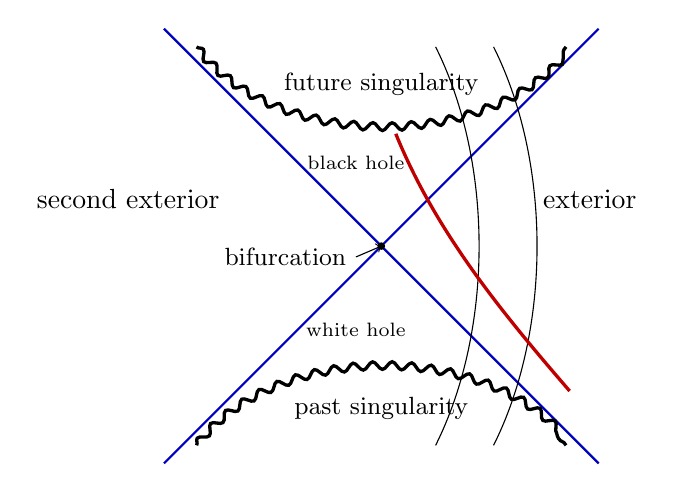
\begin{tikzpicture}[scale=0.92]
\draw[blue!75!black,thick] (-3,-3) -- (3,3);
\draw[blue!75!black,thick] (-3,3) -- (3,-3);
\draw[very thick,decorate,decoration={snake,amplitude=1.4pt,segment length=7pt}]
  (-2.55,2.75) .. controls (-1.45,1.35) and (1.45,1.35) .. (2.55,2.75);
\draw[very thick,decorate,decoration={snake,amplitude=1.4pt,segment length=7pt}]
  (-2.55,-2.75) .. controls (-1.45,-1.35) and (1.45,-1.35) .. (2.55,-2.75);
\draw (0.75,-2.75) .. controls (1.55,-1.15) and (1.55,1.15) .. (0.75,2.75);
\draw (1.55,-2.75) .. controls (2.35,-1.15) and (2.35,1.15) .. (1.55,2.75);
\draw[red!75!black,very thick] (2.6,-2.0) .. controls (1.65,-0.9) and (0.75,0.2) .. (0.2,1.55);
\fill (0,0) circle (1.5pt);
\node[above,font=\small] at (0,1.95) {future singularity};
\node[below,font=\small] at (0,-1.95) {past singularity};
\node[right] at (2.10,0.65) {exterior};
\node[left] at (-2.10,0.65) {second exterior};
\node[font=\scriptsize] at (-0.35,1.15) {black hole};
\node[font=\scriptsize] at (-0.35,-1.15) {white hole};
\node[font=\small,anchor=east] (bifurcation-label) at (-0.35,-0.15) {bifurcation};
\draw[->,thin] (bifurcation-label.east) -- (0,0);
\end{tikzpicture}
\caption{经过整理的未紧致化因果图。零测地视界在分叉面上相交；类空奇点位于未来与过去的楔形区域内。}
\end{figure}

\subsection{可能并不等于典型}

微观力学在极好的近似下具有时间反演不变性，然而宏观历史却有一个优先的方向。炸弹很容易爆炸；散落的碎片几乎从不会重新聚拢来把它重建起来。球很容易从一个不稳定的顶点滚下；一个随机抛出的球几乎从不会恰好停在那里。摆成三角形的台球很容易散开，而散开的球不会自发地排列成球架。冰块在热水中融化，而水几乎从不会吐出一个新组装好的冰块。

区别在于熵。低熵宏观态只占据相空间中极小的区域；高熵宏观态则包含数量巨大的微观排列。方程允许反向的轨迹，但要制备其初始微观态需要极其精确的关联。

\begin{classroomqa}
\audiencequestion{难道每一个精确的散射构型不都与精确的时间反演构型同样不可能吗？\lecturetimestamp{00:56:55}}
\lecturerresponse{对于逐个指定的微观态而言，是的。当我们比较宏观态时，不对称性才出现。一个散射的排列所包含的微观态远多于一个精确组装好的三角形，因此几乎每一个与第一种描述相容的微观态在宏观上仍然是无序的。}
\end{classroomqa}

一个发射出完全组织化的Alice的白洞，就是这种降低熵的历史在引力上的版本。可逆方程允许它，但它需要一个极其特殊的过去。视界本身携带熵和隐藏的微观信息，因此一个Alice大小的涨落并非逻辑上被禁止；它只是被压倒性地抑制了。

\begin{classroomqa}
\audiencequestion{这样的涨落是量子力学的还是热学的？\lecturetimestamp{00:59:48}}
\lecturerresponse{两种都可以有贡献。在普通的热系统中，主导的语言是热涨落；对于黑洞，量子效应与热效应交织在一起。无论哪种情况，核心的抑制都是熵性的。}
\end{classroomqa}

\section{固有距离与Penrose紧致化}

在绘制整体时空之前，我们应当把径向的术语精确化。固有时是时钟沿类时世界线所测量的量。固有距离是一系列局域米尺沿选定的类空曲线所测量的量。对于Schwarzschild的常\(t\)切片，
\begin{equation}
d\rho=\frac{dr}{\sqrt{1-2GM/r}}.
\label{eq:l04-proper-distance}
\end{equation}
因此\(r\)是一个面积坐标，而不是从视界出发的直接米尺距离。

现在从径向平直时空开始。只保留\(t\)和\(\rho\ge0\)。线\(\rho=0\)是空间原点，一条进入原点的径向光线在相反的一侧物理上继续向外传播，这在约化半平面中表现为一次反射。

Penrose图把\(t\)和\(\rho\)的所有有限与无限取值映射到一个有限区域，同时保持零方向。它的两条规则是：
\begin{enumerate}
\item 把整个时空紧致化到一个有限区域；
\item 保持径向光线在\(45^\circ\)。
\end{enumerate}
长度和普通角度被扭曲；因果关系则不然。

\begin{figure}[htbp]
\centering
\includegraphics[width=0.70\textwidth]{lecture_04_figure_06.png}
\caption{径向Minkowski时空的完整紧致化网格。无限时间位于左上和左下的端点，无限半径被压缩到右侧的尖端。}
\lectureframe{01:14:44.040}
\end{figure}

\begin{figure}[htbp]
\centering
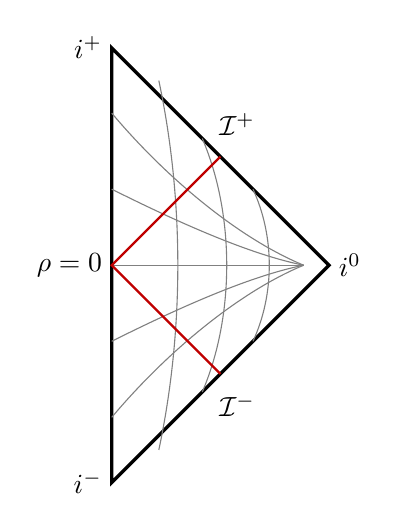
\begin{tikzpicture}[scale=0.92]
\coordinate (im) at (0,-3);
\coordinate (ip) at (0,3);
\coordinate (iz) at (3,0);
\draw[very thick] (im) -- (ip) -- (iz) -- cycle;
\draw[gray] (0,-2.1) .. controls (0.8,-1.15) and (1.8,-0.35) .. (2.65,0);
\draw[gray] (0,-1.05) .. controls (0.9,-0.6) and (1.9,-0.15) .. (2.65,0);
\draw[gray] (0,0) -- (2.65,0);
\draw[gray] (0,1.05) .. controls (0.9,0.6) and (1.9,0.15) .. (2.65,0);
\draw[gray] (0,2.1) .. controls (0.8,1.15) and (1.8,0.35) .. (2.65,0);
\draw[gray] (0.65,-2.55) .. controls (1.0,-0.9) and (1.0,0.9) .. (0.65,2.55);
\draw[gray] (1.25,-1.75) .. controls (1.7,-0.7) and (1.7,0.7) .. (1.25,1.75);
\draw[gray] (1.95,-1.05) .. controls (2.25,-0.4) and (2.25,0.4) .. (1.95,1.05);
\draw[red!75!black,thick] (1.5,-1.5) -- (0,0) -- (1.5,1.5);
\node[left] at (ip) {\(i^+\)};
\node[left] at (im) {\(i^-\)};
\node[right] at (iz) {\(i^0\)};
\node[above right] at (1.35,1.65) {\(\mathcal{I}^+\)};
\node[below right] at (1.35,-1.65) {\(\mathcal{I}^-\)};
\node[left] at (0,0) {\(\rho=0\)};
\end{tikzpicture}
\caption{有限三角形中的径向Minkowski时空。红色光线从\(\mathcal{I}^-\)进入，到达原点，并从\(\mathcal{I}^+\)离开。}
\label{fig:l04-flat-penrose}
\end{figure}

这些端点具有不同的因果含义：
\begin{equation}
\begin{aligned}
i^-&:\ \text{past timelike infinity},\\
i^+&:\ \text{future timelike infinity},\\
i^0&:\ \text{spatial infinity},\\
\mathcal{I}^-&:\ \text{past null infinity},\\
\mathcal{I}^+&:\ \text{future null infinity}.
\end{aligned}
\end{equation}
符号\(\mathcal{I}^{-}\)和\(\mathcal{I}^{+}\)读作scri minus和scri plus。

\begin{classroomqa}
\audiencequestion{光线是否应当穿过每个被扭曲的网格单元的角点，从而略微弯曲？\lecturetimestamp{01:11:08}}
\lecturerresponse{如果完整地画出坐标网格，其交点会与零曲线一致。关键的构造是共形的：径向零方向保持在\(45^\circ\)，尽管常\(t\)和常\(\rho\)的网格线会弯曲并变得密集。}
\end{classroomqa}

\begin{classroomqa}
\audiencequestion{如果光线没有射向原点，该如何绘制它？\lecturetimestamp{01:11:45}}
\lecturerresponse{它会到达一个非零的最近接近距离，然后向外返回。一旦保留了角向运动，其投影的径向路径就不必是一条单一的直线\(45^\circ\)。}
\end{classroomqa}

\begin{classroomqa}
\audiencequestion{那么为什么那条光线不在\(45^\circ\)处？\lecturetimestamp{01:12:49}}
\lecturerresponse{\(45^\circ\)规则是针对径向光线陈述的。携带角动量的零测地线将其部分运动用于角方向，因此它在\(t\)-\(\rho\)平面上的投影不是径向的。}
\end{classroomqa}

\section{永恒史瓦西图}

紧致化后的图有四个区域。其两侧的菱形是渐近平直的外部区域。上方的三角形是黑洞内部，终止于未来类空奇点。下方的三角形是白洞区域，起始于过去类空奇点。这些区域共同构成了最大延拓的史瓦西几何。

\begin{figure}[htbp]
\centering
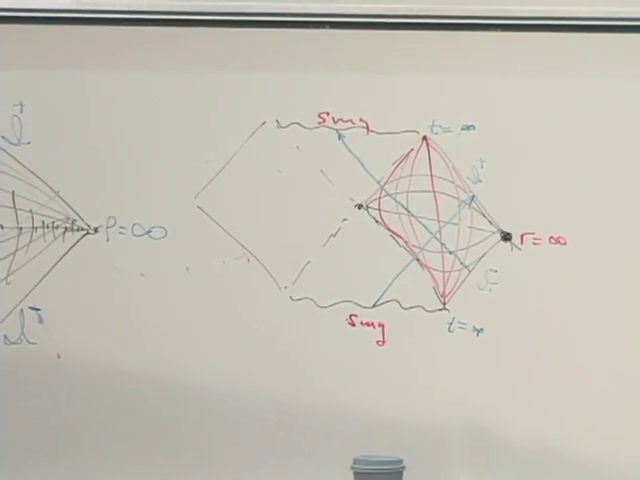
\includegraphics[width=0.74\textwidth]{lecture_04_figure_07.png}
\caption{黑板上画出的完整永恒史瓦西彭罗斯图，标有奇点、视界、零测地线以及一个渐近边界。}
\lectureframe{01:21:30.000}
\end{figure}

\begin{figure}[htbp]
\centering
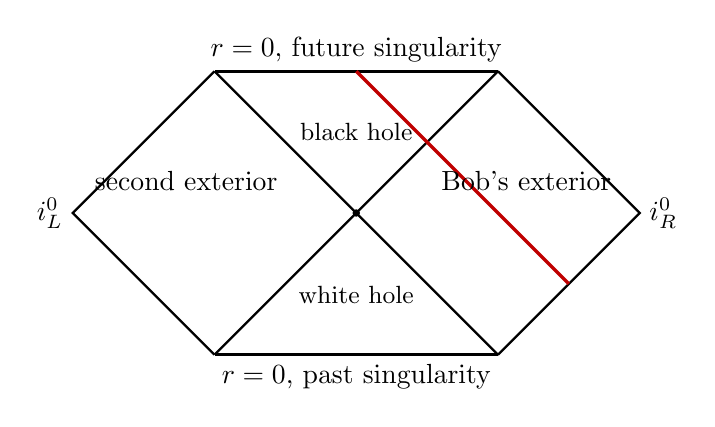
\begin{tikzpicture}[scale=0.90]
\coordinate (C) at (0,0);
\coordinate (TL) at (-2,2);
\coordinate (TR) at (2,2);
\coordinate (BL) at (-2,-2);
\coordinate (BR) at (2,-2);
\coordinate (L) at (-4.0,0);
\coordinate (R) at (4.0,0);
\draw[very thick] (TL) -- (TR);
\draw[very thick] (BL) -- (BR);
\draw[thick] (C) -- (TL) (C) -- (TR) (C) -- (BL) (C) -- (BR);
\draw[thick] (TL) -- (L) -- (BL);
\draw[thick] (TR) -- (R) -- (BR);
\draw[red!75!black,very thick] (3,-1) -- (1,1) -- (0,2);
\node[above] at (0,2) {\(r=0\), future singularity};
\node[below] at (0,-2) {\(r=0\), past singularity};
\node[font=\small] at (0,1.15) {black hole};
\node[font=\small] at (0,-1.15) {white hole};
\node at (2.4,0.45) {Bob's exterior};
\node at (-2.4,0.45) {second exterior};
\node[right] at (R) {\(i^0_R\)};
\node[left] at (L) {\(i^0_L\)};
\fill (C) circle (1.5pt);
\end{tikzpicture}
\caption{永恒史瓦西的四个区域。一条入射径向光线穿过未来视界并终止于\(r=0\)。}
\label{fig:l04-eternal}
\end{figure}

一条来自\(\mathcal{I}^-\)的入射径向光线穿过未来视界并终止于奇点。上方三角形中的每一条因果曲线都有同样的命运。第二个外部区域常被描述为爱因斯坦--罗森桥的另一端开口，但它不可穿越：任何从一个外部区域到另一个外部区域的因果旅行尝试都会进入黑洞区域并到达奇点。

\begin{classroomqa}
\audiencequestion{两个外部世界是否由虫洞连接，能否通过它发送信号？\lecturetimestamp{01:22:21}}
\lecturerresponse{永恒几何在适当的空间切片上包含一个爱因斯坦--罗森桥，但没有因果信号能从一个外部区域穿越到另一个外部区域。桥收缩得太快；甚至进入视界的光也会终止于未来奇点。}
\end{classroomqa}

这张图描述的是一个自始至终存在的洞。真实的的天体物理黑洞由坍缩物质形成。它们的因果图没有过去的白洞奇点，也没有第二个渐近外部区域。要构造那种几何，我们需要理解球壳。

\section{通过坍缩制备黑洞}

想象一个由入射粒子组成的弥散球壳。它们可以是光子：能量产生引力，因此足够集中的辐射脉冲可以形成黑洞。坍缩之前，中心区域类似于空的平直时空；在足够能量被压缩之后，外部区域类似于史瓦西。任务是在移动的球壳两侧衔接这些区域。

\subsection{牛顿球壳定理}

对于总质量为\(M\)的球对称牛顿球壳，引力的高斯定律为
\begin{equation}
\oint \mathbf{g}\cdot d\mathbf{A}=-4\pi G M_{\mathrm{enc}}.
\label{eq:l04-gauss-gravity}
\end{equation}
球对称性使得\(\mathbf{g}=g(r)\hat{\mathbf r}\)，因此
\begin{equation}
g(r)=
\begin{cases}
0, & r<R_{\mathrm{shell}},\\[4pt]
-\dfrac{GM}{r^2}, & r>R_{\mathrm{shell}}.
\end{cases}
\label{eq:l04-shell-field}
\end{equation}
在内部，没有质量被包围，引力场消失。在外部，球壳的作用完全等同于位于中心的点质量\(M\)。内部的势是常数而非零，但不再存在局部牛顿力。\editorialnote{课堂上给出的场线论证被高斯定律精确地捕捉。零场与常数势之间的区别在比较相对论中的时钟归一化时很重要。}

只要总质量守恒，当一个完美球对称的球壳收缩时，该结论仍然成立。只有内部解与外部解之间边界的位置发生变化。

\subsection{伯克霍夫定理}

相对论对应物是伯克霍夫定理：每一个球对称真空区域局部地是史瓦西族的一部分。对于中心没有质量的球壳，
\begin{align}
ds^2_{\mathrm{inside}}&=-dT^2+dR^2+R^2d\Omega_2^2,\\
ds^2_{\mathrm{outside}}&=
-\left(1-\frac{2GM}{r}\right)dt^2
\nonumber\\
&\quad+\frac{dr^2}{1-2GM/r}
+r^2d\Omega_2^2.
\label{eq:l04-birkhoff-pieces}
\end{align}

\begin{figure}[htbp]
\centering
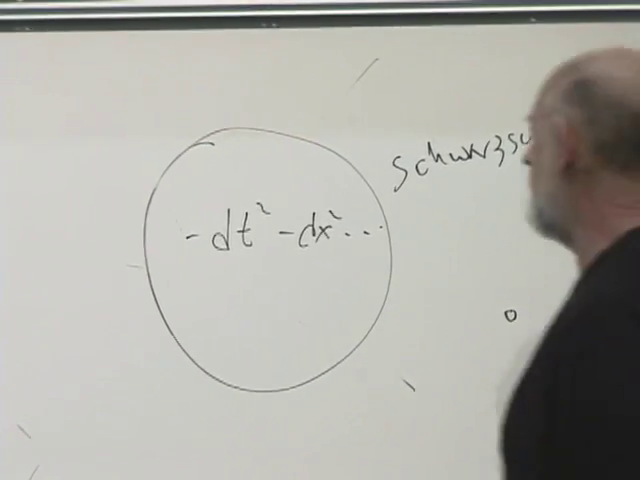
\includegraphics[width=0.74\textwidth]{lecture_04_figure_08.png}
\caption{球壳衔接图：圆内为平直时空，圆外为史瓦西解。}
\lectureframe{01:34:15.000}
\end{figure}

\begin{classroomqa}
\audiencequestion{在广义相对论中，球壳外部出现什么度规？\lecturetimestamp{01:33:17}}
\lecturerresponse{史瓦西度规，其质量参数等于球壳的总守恒质量。空的中心区域局部地是闵可夫斯基时空。}
\end{classroomqa}

\begin{classroomqa}
\audiencequestion{如果壳层收缩，为什么质量参数不改变？\lecturetimestamp{01:34:33}}
\lecturerresponse{因为总能量守恒。壳层的半径以及动能或束缚能贡献可能改变，但对于孤立球对称系统，守恒的外部质量是固定的。运动壳层改变的是平坦区域与施瓦西区域相连接的位置。}
\end{classroomqa}

内部平坦并不意味着内部时钟必然与无穷远处的时钟具有相同的归一化。跨壳层匹配可以将内部时间坐标乘以一个常数，而运动壳层需要相应的连接条件。\editorialnote{伯克霍夫定理在局部固定每个真空区域。它们坐标之间的整体关系由跨壳层匹配诱导度规和外曲率确定。这些细节被推迟，正如坍缩构造被推迟到下一讲一样。}

我们现在拥有形成所需的两个部分：收缩壳层内部的闵可夫斯基时空和其外部的施瓦西时空。当壳层向内运动时，它们的界面描绘出一个世界管。沿着该世界管穿过原本的施瓦西半径，将用规则的坍缩前区域取代图~\ref{fig:l04-eternal}中非物理的过去半部分，并揭示真实黑洞的事件视界从何处开始。
